\subsection{Particelle doppie}

\begin{figure}
	\centering
	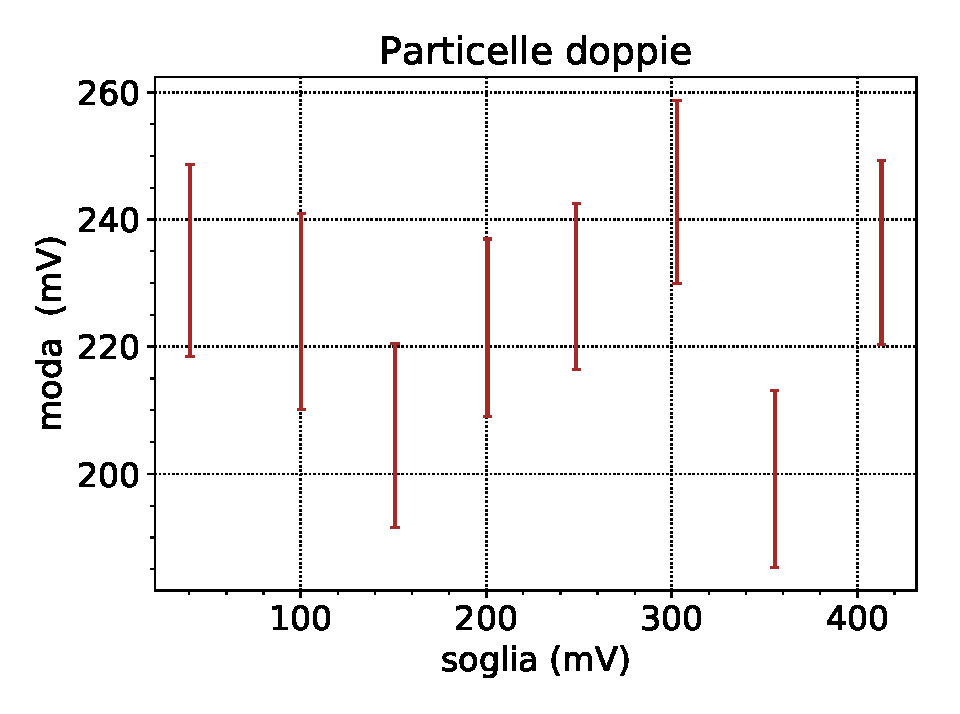
\includegraphics[width=23em]{doppie}
	\caption{Moda della distribuzione del rilascio di energia nel PM5
	negli eventi in coincidenza PM4 \& PM5
	in funzione della soglia del PM4.}
	\label{corre}
\end{figure}

\begin{figure}
	\centering
	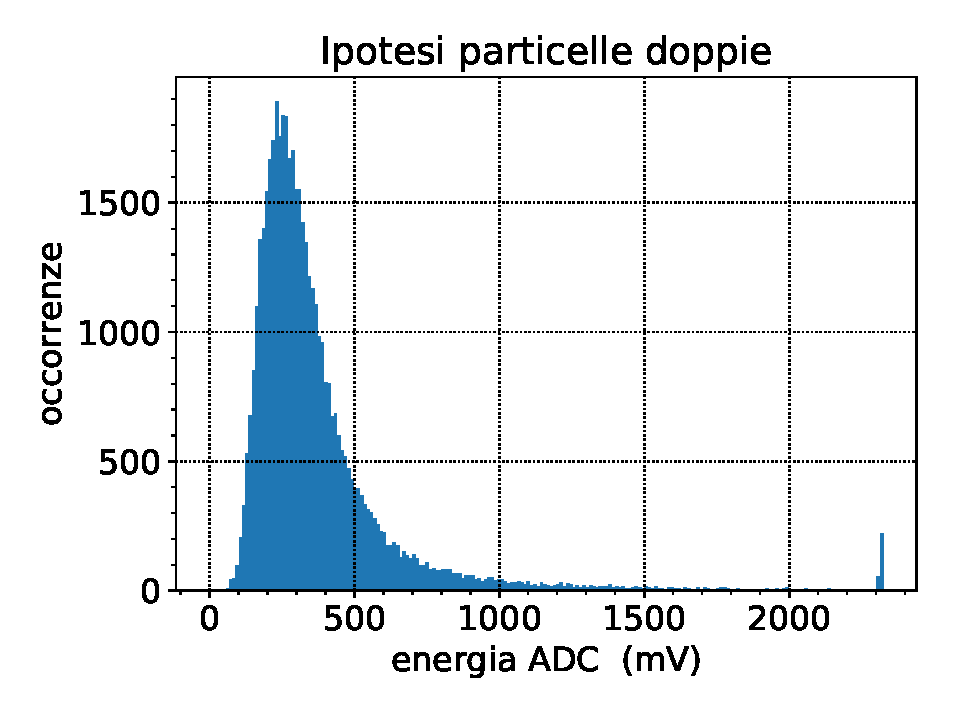
\includegraphics[width=23em]{nuovo}
	\caption{Spettro del rilascio di energia sul PM6 sulla coincidenza 1\&6.
	I bin sono opportunamente allineati rispetto ai canali dell'ADC.}
	\label{nuovo}
\end{figure}

Se la distribuzione dell'energia rilasciata è abbastanza stretta
ci aspettiamo di osservare una distribuzione bimodale,
con una moda circa doppia dell'altra,
nel caso in cui ci sia un passaggio frequente di 2 particelle nello stesso momento.
Studiamo lo spettro dei rilasci di energia della configurazione 1\&6,
in quanto gli angoli selezionati da tale scelta variano di meno di quelli selezionati dalle altre configurazioni;
in questo modo minimizziamo la larghezza della distribuzione.
I dati usati sono gli stessi dell'istogramma 1\&6 in \autoref{isto}.
Riportiamo un nuovo istogramma in \autoref{nuovo},
avendo cura di allineare i bin in modo da avere una quantità fissata di canali dell'ADC per ogni bin.
% La moda calcolata con l'istogramma è \SI{232\pm11}{mV}.

Poiché in \autoref{nuovo} non osserviamo due mode,
proviamo con una strategia meno diretta.
Studiamo la distribuzione dell'energia rilasciata nel PM5,
per gli eventi in coincidenza 4\&5,
in funzione della soglia del PM4.
Un'eventuale presenza di eventi con particelle doppie,
quindi con distribuzione dell'energia rilasciata diversa,
provoca un cambiamento della distribuzione misurata in funzione della soglia.
Il PM5 ha la soglia più bassa possibile (\SI{30}{mV}) per mantenere minima la selezione.
La moda (calcolata con gli istogrammi) è riportata in \autoref{corre} in funzione della soglia.

Dalla \autoref{corre} non si nota un andamento.
Se avessimo avuto a disposizione due amplificatori
avremmo potuto analizzare le correlazioni temporali tra rilasci elevati di energia in due scintillatori diversi.

